\graphicspath{{./chapters/chapter06/}}
\chapter{Основы тестирования}

В этой главе мы проверяем гипотезы о неизвестном параметре $\vartheta$. Как и ранее, мы рассматриваем статистический эксперимент $(\mathcal{X}, \mathcal{B}, \mathcal{P})$, где $\mathcal{P}=\{ P_\vartheta \mid \vartheta \in \Theta \}$.

\begin{exmp}
	Обсудим (упрощенный) клинический эксперимент, в которомы мы принимаем решение, лучше ли новоизобретенное лекарство B, чем известное лекарство А или нет. Предположим, что мы знаем по опыту предыдущих лет, что А имеет шанс излечения 65\%. Новое лекарство B было протестировано на 100 подопытных и 80\% выздоровели. Должны мы выбрать A или B? \\
	На языке математики мы проверяем:
	\[ H: p \leq 0.65 \quad \text{против} \quad K: p > 0.65, \]
	где $p$ -- неизвестная вероятность излечения после принятия лекарства B.
\end{exmp}

\begin{defn}
	Пусть $\Theta = \Theta_H \cup \Theta_K$  -- разделение параметрического пространства.
	\begin{enumerate}
		\item $\Theta_H$ называется \textbf{\textit{(нулевой) гипотезой}}, $\Theta_K$ называется \textbf{\textit{альтернативой}}.
		\item \textbf{\textit{Рандомизированный критерий}} -- измеримое отображение
		\[ \varphi:(\mathcal{X}, \mathcal{B}) \rightarrow ([0, 1], \mathcal{B}|_{[0,1]}). \]
		Функция $\varphi(x)$ -- это вероятность принятия решения, что $\vartheta \in \Theta_K$, после наблюдения $x=X(\omega)$. Множество таких критериев обозначим:
		\[ \Phi = \{ \varphi \mid \varphi \text{ -- рандомизированный критерий} \}. \]
		\item Для критерия $\varphi$ назовем $\mathcal{K}= \{x \mid \varphi(x)=1 \}$ \textbf{\textit{критической областью}}, а $\mathcal{R}= \{x \mid \varphi(x) \in (0,1) \}$ -- \textbf{\textit{областью рандомизации}}. Критерий $\varphi$ называется \textbf{\textit{нерандомизированным}}, если $\mathcal{R} = \emptyset$. 
	\end{enumerate}
\end{defn}

\begin{exmp} \label{exmp6.3}
	В ситуации в предыдущем примере мы знаем, что $\overline{X}_n$ является UMVU-оценкой $p$. Разумно принять $K$, если значение $\overline{X}_n$ достаточно большое, например:
	\[ \varphi(x) =
	\left \{
	\begin{array}{cl}
	1 & \overline{X}_n > 0.7 \\
	0 & \overline{X}_n \leq 0.7 
	\end{array}
	\right.
	\] 
	является разумным критерием.
\end{exmp}

\begin{rmrk}
	При принятии решения могут произойти две ошибки:
	\begin{itemize}
		\item Ошибка первого рода: отклонить гипотезу $H$, когда она верна.
		\item Ошибка второго рода: принять гипотезу $H$, когда она неверна.
	\end{itemize}
	\begin{center}
		\quad\quad\quad\quad\quad\quad\quad Истина \\
		Решение
		\begin{tabular}{| c | c | c|}
			\hline
			& $\Theta_H$ & $\Theta_K$ \\
			\hline
		 $\Theta_H$ & \checkmark & Ошибка 2-го рода \\
		\hline
			 $\Theta_K$ & Ошибка 1-го рода & \checkmark \\
			 \hline
		\end{tabular}
	\end{center}
	Обе ошибки могут произойти с определенными вероятностями.
\end{rmrk}

\begin{exmp}
	В Примере \ref{exmp6.3} вероятность принятия $K$:
	\[ P_p(\varphi(X)=1)=P_p(\overline{X}_n > 0.7). \]
	На практике биномиальное распределение можно аппроксимировать нормальным:
	\[
	\begin{aligned}
	P_p(\overline{X}_n > 0.7) & = P_p\bigg(\frac{\sqrt{n}(\overline{X}_n - p)}{\sqrt{p(1-p)}} > \frac{\sqrt{n}(0.7 - p)}{\sqrt{p(1-p)}}\bigg) \\
	\text{ЦПТ} \rightarrow & \approx P\bigg(\mathcal{N}(0,1) > \frac{\sqrt{n}(0.7 - p)}{\sqrt{p(1-p)}}\bigg) = \Phi\bigg(\frac{\sqrt{n}(0.7 - p)}{\sqrt{p(1-p)}}\bigg).
	\end{aligned}	 
	\]
	Используя Лемму Слуцкого, мы можем заменить $p$ на $\overline{X}_n$ в знаменателе. Пусть $n=100$ и $\overline{X}_n = 0.8$, тогда
	\[ P_p(\varphi(X)=1) \approx \Phi(25(p-0.7)).  \]
	Например, если $p \leq 0.65$:
	\[ P_p(\text{Ошибка первого рода}) \approx
	\left \{
	\begin{array}{cl}
	0, & p = 0.5 \\
	0.006, &  p = 0.6
	\end{array}
	\right.
	\]
	Вероятность ошибки ограничена сверху:
	\[ P_p(\text{Ошибка первого рода}) \leq P_{0.65}(\text{Ошибка первого рода}) \approx \Phi(1.25) \approx 0.106. \]
	Симметрично
	\[ P_p(\text{Ошибка второго рода}) \approx
	\left \{
	\begin{array}{cl}
	0, & p = 0.9 \\
	0.006, &  p = 0.8 \\
	0.5, & p = 0.7
	\end{array}
	\right.
	\]
	Граница сверху:
	\[ P_p(\text{Ошибка второго рода}) \leq P_{0.65}(\text{Ошибка второго рода}) \approx 0.894. \]
\end{exmp}

\begin{rmrk}
	В идеале, мы хотим минимизировать вероятности обеих ошибок и выбрать оптимальный критерий. Проблема заключается в том, что критерии
	\[ \varphi_0(X) \equiv 0 \Rightarrow
	\left \{
	\begin{array}{cl}
	P_p(\text{Ошибка первого рода}) = 0 \\
	P_p(\text{Ошибка второго рода}) = 1
	\end{array}
	\right.
	\]
	\[ \varphi_1(X) \equiv 1 \Rightarrow
	\left \{
	\begin{array}{cl}
	P_p(\text{Ошибка первого рода}) = 1 \\
	P_p(\text{Ошибка второго рода}) = 0
	\end{array}
	\right.
	\]
	являются оптимальными, если нужно минимизировать вероятность одной из ошибок, но не минимизирует вероятности обеих ошибок одновременно. На практике берут границу $\alpha$ для вероятности ошибки первого рода и минимизируют вероятность ошибки второго рода по всем критериям. Обычно $0.01 \leq \alpha \leq 0.1$. 
\end{rmrk}

\begin{defn}
	Пусть $\varphi$ -- критерий для $H: \varphi \in \Theta_H \text{ против } K:\vartheta \in \Theta_K$.
	\begin{enumerate}
		\item Функция
		\[ \beta_\varphi:
		\left \{
		\begin{array}{ccl}
        \Theta & \rightarrow & [0, 1] \\
		\vartheta & \mapsto & \ME_\vartheta[\varphi(X)]
		\end{array}
		\right.
		\]
		называется \textbf{\textit{функцией мощности $\varphi$}}.
		\item Критерий $\varphi$ называется \textbf{\textit{критерием с уровнем значимости $\alpha$}} $\in [0, 1]$, если
		\[ \beta_\varphi(\vartheta) \leq \alpha \quad \forall \vartheta \in \Theta_H \]
		Зададим множество таких критериев:
		\[ \Phi_\alpha = \{ \varphi \in \Phi \ |\ \varphi \text{ -- критерий с уровнем значимости }\alpha  \}. \]
		\item Критерий $\varphi$ называется \textbf{\textit{несмещенным с уровнем значимости $\alpha$}} $\in [0, 1]$, если $\varphi \in \Phi_\alpha$ и
		\[ \beta_\varphi(\vartheta) \geq \alpha \quad  \forall \vartheta \in \Theta_K, \]
		\[  \Phi_{\alpha \alpha} = \{ \varphi  \in \Phi_\alpha \ |\ \varphi \text{ -- несмещенный критерий}  \}. \]
	\end{enumerate}
\end{defn}

\begin{rmrk} \
	\begin{enumerate}
		\item Если $\varphi$ -- нерандомизированный критерий, то
		\[ \beta_\varphi(\vartheta) = P_\vartheta(\varphi(X) = 1) \]
		-- вероятность принятия $K$. В частности,
		\begin{enumerate}
			\item $\vartheta \in \Theta_H$: $\beta_\varphi(\vartheta)$ -- вероятность ошибки 1-го рода.
			\item $\vartheta \in \Theta_K$: $1-\beta_\varphi(\vartheta)$ -- вероятность ошибки 2-го рода.
		\end{enumerate}
		Аналогичная интерпретация имеет место для радномизированных критериев.
		\item Критерий $\varphi$ ограничивает вероятность ошибки первого рода уровнем значимости $\alpha$ $\forall \vartheta \in \Theta_H$.
		\item Для несмещенного критерия $\varphi$ вероятность принятия гипотезы $K$ в случае, если $\vartheta \in \Theta_K$, не меньше, чем в случае, если $\vartheta \in \Theta_H$.
	\end{enumerate}
\end{rmrk}

\begin{exmp}
	Функция мощности критерия из Примера \ref{exmp6.3} будет приблизительно равна:
	\[ \beta_\varphi:
	\left \{
	\begin{array}{ccl}
	[0, 1] & \rightarrow & [0, 1] \\
	p & \mapsto & \beta_\varphi(p) \approx \Phi\Big(\frac{\sqrt{n}(p-0.7)}{\sqrt{\overline{X}_n (1-\overline{X}_n)}}\Big).
	\end{array}
	\right.
	\]
	Уровень значимости критерия $\varphi$: $\alpha \approx 0.106$.
\end{exmp}

\begin{defn} \
	\begin{enumerate}
		\item Критерий $\varphi^* \in \Phi_\alpha$ называется \textbf{\textit{равномерно наиболее мощным (UMP) с уровнем значимости $\alpha$}}, если
		\[\beta_{\varphi^*}(\vartheta) = \sup_{\varphi \in \Phi_\alpha} \beta_\varphi(\vartheta) \quad \forall \vartheta \in \Theta_K. \]
		\item Критерий $\varphi^* \in \Phi_{\alpha \alpha}$ называется \textbf{\textit{равномерно наиболее мощным несмещенным (UMPU) с уровнем значимости $\alpha$}}, если
		\[\beta_{\varphi^*}(\vartheta) = \sup_{\varphi \in \Phi_{\alpha\alpha}} \beta_\varphi(\vartheta) \quad \forall \vartheta \in \Theta_K. \]
	\end{enumerate}
\end{defn}

\begin{thm} \label{thm6.11}
	Пусть $\mathcal{P} = \{P_\vartheta\ |\ \vartheta \in \Theta  \}$ -- семейство распределений на $(\mathcal{X}, \mathcal{B})$, статистика $T:(\mathcal{X}, \mathcal{B}) \rightarrow (\mathcal{T}, \mathcal{D})$ -- достаточная для $\vartheta$ и $\varphi$ -- критерий. Тогда существует критерий $\psi \circ T$, обладающий той же функцией мощности, что и $\varphi$, а именно:
	\[ \psi \circ T = \ME[\varphi | T]. \]
\end{thm}
\begin{proof}
	Пусть $\psi(t) = \ME[\varphi | T = t]$. Во-первых, $\psi(T) \in [0, 1]$, так как это критерий. Также,
	\[ \beta_{\psi \circ T}(\vartheta) = \ME_\vartheta[\psi \circ T] = \ME_\vartheta[\ME[\varphi | T ]] = \ME_\vartheta[\varphi] = \beta_\varphi(\vartheta). \]
\end{proof}

\begin{rmrk} \
	\begin{enumerate}
		\item Теорема \ref{thm6.11} показывает, что для создания критерия всегда можно воспользоваться достаточной статистикой.
		\item Простейший случай простых гипотез:
		\[ H:\vartheta \in \{\vartheta_0 \}\quad \text{против} \quad K:\vartheta \in \{\vartheta_1 \}, \quad \vartheta_0 \neq \vartheta_1. \]
		Зададим доминирующую меру для $P_{\vartheta_0}$ и $P_{\vartheta_1}$:
		\[\mu = P_{\vartheta_0} + P_{\vartheta_1}. \]
		Также, пусть
		\[ p_i = \frac{dP_{\vartheta_i}}{d\mu} \]
		и 
		\[ \frac{p_1}{p_0} = 
		\left \{
		\begin{array}{cl}
		\infty, & p_1 > 0, p_0 = 0 \\
		\text{произвольное}, & p_1 = 0, p_0 = 0.
		\end{array}
		\right.
		\]
		Имеют место следующие утверждения:
		\begin{enumerate}
			\item Величина $\frac{p_1}{p_0}$ независима от $\mu$ (вплоть до множеств меры нуль).
			\item $\frac{p_1}{p_0}$ -- минимальная достаточная статистика для $\vartheta$ (Пример \ref{exmp4.20}).
			\item UMP-критерий с уровнем значимости $\alpha$ максимизирует
			\[ \beta_\varphi(\vartheta_1) = \ME_{\vartheta_1}[\varphi(X)] = \int \varphi(x) p_1(x) \mu(dx) \]
			при ограничении
			\[ \beta_\varphi(\vartheta_0) = \ME_{\vartheta_0}[\varphi(X)] = \int \varphi(x) p_0(x) \mu(dx) \leq \alpha. \]
		\end{enumerate}
	\end{enumerate}
\end{rmrk}

\begin{defn}
	В случае простой гипотезы критерий $\varphi$ называется \textbf{\textit{критерием Неймана-Пирсона (NP критерий)}}, если существует константа $c \in [0,\infty )$, такая что
	\[ \varphi(x):
	\left \{
	\begin{array}{cl}
	1, & p_1(x) > cp_0(x), \\
	0, & p_1(x) < cp_0(x).
	\end{array}
	\right.
	\]
\end{defn}

\begin{thm}[\textbf{\textit{NP лемма}}]
	Пусть $\Theta = \{ \vartheta_0, \vartheta_1 \}$ и рассматриваются гипотезы
	\[ H:\vartheta \in \{\vartheta_0 \}\quad \text{против} \quad K:\vartheta \in \{\vartheta_1 \}. \]
	\begin{enumerate}
		\item NP критерий $\varphi^*$ -- UMP-критерий с уровнем значимости $\alpha = \ME_{\vartheta_0}[\varphi^*(X)]$.
		\item Для любого $\alpha \in [0, 1]$ существует NP критерий $\varphi$, такой что $\ME_{\vartheta_0}[\varphi(X)] = \alpha$.
		\item Если $\varphi'$ -- UMP-критерий с уровнем значимости $\alpha$, то $\varphi'$ -- (п.н.) NP критерий. Если $\ME_{\vartheta_0}[\varphi'(X)] < \alpha$, то $\ME_{\vartheta_1}[\varphi'(X)]=1$.
	\end{enumerate}
\end{thm}
\begin{proof}
	\begin{enumerate}
		\item Пусть $\varphi^*$ -- NP критерий с константой $c^*$ и $\varphi$ -- другой критерий, такой что $\beta_\varphi(\vartheta_0) \leq \alpha = \beta_{\varphi^*}(\vartheta_0)$. Рассмотрим
		\[ \beta_{\varphi^*}(\vartheta_1) - \beta_\varphi(\vartheta_1) = \int (\varphi^* - \varphi) p_1 d\mu = \int (\varphi^* - \varphi)(p_1 - c^*p_0)d\mu + \int c^* p_0 (\varphi^* - \varphi) d\mu. \]
		Второй интеграл неотрицателен, так как его подинтегральное выражение: 
		\[c^*(\beta_{\varphi^*}(\vartheta_0) - \beta_\varphi(\vartheta_0)) \geq 0.\]
		 В первом интеграле:
		\[\varphi^* - \varphi > 0 \Longrightarrow \varphi^* > 0 \Longrightarrow p_1 \geq c^*p_0, \]
		\[\varphi^* - \varphi < 0 \Longrightarrow \varphi^* < 1 \Longrightarrow p_1 \leq c^*p_0 \]
		$\Longrightarrow (\varphi^* - \varphi)(p_1 - c^*p_0) \geq 0$ всегда.
		\item Для $c \in \MR$ зададим
			\begin{center}\centering
				\begin{minipage}{0.18\textwidth}
					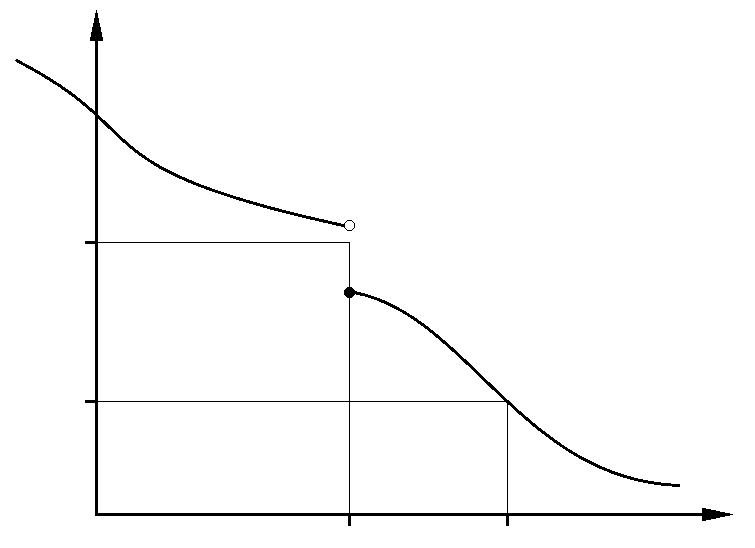
\includegraphics[width=\linewidth, right]{alpha}
					\captionsetup{labelformat=empty}
					\put (-90,32) {$\displaystyle \alpha_1 $}
					\put (-90,12) {$\displaystyle \alpha_2 $}
					\put (-49,-5) {$\displaystyle c_1 $}
					\put (0,-5) {$\displaystyle c $}
			        \put (-30,-5) {$\displaystyle c_2$}
					\put (-90,65) {$\displaystyle \alpha$}
				\end{minipage}
				\begin{minipage}{0.7\textwidth}
					\[ \alpha(c) := P_{\vartheta_0}\Big( \frac{p_1(X)}{p_0(X)} > c \Big). \]
					Очевидно, что $1 - \alpha(c)$ -- функция распределения. Для $\alpha \neq 0$ выберем $c^*$ таким образом, чтобы выполнялось соотношение
					\[ \alpha(c^*) \leq \alpha \leq \alpha(c^*-), \]
				\end{minipage}
			\end{center}
		где $\alpha(c-)$ обозначает левый предел в точке $c$. Для $\alpha = 0$ пусть $c^* = \infty$. Зададим функции
		\[ \gamma^*:
		\left \{
		\begin{array}{cl}
		\frac{\alpha - \alpha(c^*)}{\alpha(c^*-)-\alpha(c^*)}, & \text{если $\alpha(c^*-)-\alpha(c^*) > 0$}, \\
		0, & \text{иначе}.
		\end{array}
		\right.
		\]
		и
		\[ \varphi^*(x):
		\left \{
		\begin{array}{cl}
		1, & p_1(x) > c^* p_0(x), \\
		\gamma^*, & p_1(x) = c^*p_0(x), \\
		0, & p_1(x) < c^* p_0(x).
		\end{array}
		\right.
		\]
		Если $c^* < \infty$, то
		\[ \beta_{\varphi^*}(\vartheta_0) = \int_{\{p_1 > c^* p_0\}}dP_{\vartheta_0} + \int_{\{p_1 = c^* p_0\}}\gamma^* dP_{\vartheta_0} = \alpha(c^*)+\gamma^*(\alpha(c^*-)-\alpha(c^*)) = \alpha. \]
		Если $c^* = \infty$, то
		\[\beta_{\varphi^*}(\vartheta_0) = P_{\vartheta_0}(p_1(X) > \infty) = 0. \]
		\item Пусть $\varphi'$ -- UMP-критерий с уровнем значимости $\alpha$ и $\varphi^*$ -- критерий из (ii). Так как из (i) следует, что $\varphi^*$ -- UMP, то $\beta_{\varphi^*}(\vartheta_1) = \beta_{\varphi_1}(\vartheta_1)$. Таким образом,
		\[ \int (\varphi^* - \varphi')p_1 d\mu = 0, \]
		но
		\[
		\int (\varphi^* - \varphi')p_1 d\mu = \int (\varphi^* - \varphi')(p_1 - c^*p_0)d\mu + \int c^*p_0(\varphi^* - \varphi')d\mu = I+II \]
		Так как $\beta_{\varphi^*}(\vartheta_0)=\alpha \geq \beta_{\varphi'}(\vartheta_0)$, второй интеграл неотрицателен. Как и в доказательстве (i), мы можем показать, что $I \geq 0$. Следовательно, $I = II = 0$. Зададим множество
		\[ S= \{ x\ |\ \varphi'(x) \neq \varphi^*(x) \} \cap \{ x\ |\ p_1(x) \neq c^*p_0(x) \}. \]
		На множестве $S$ имеет место неравенство
		\[ (\varphi^* - \varphi')(p_1 - c^*p_0)>0 \]
		$\Longrightarrow \mu(S) = 0$. На его дополнении $S^c$ $\varphi'$ -- NP критерий. Так как $II = 0$, либо $c^* = 0$, либо $\beta_{\varphi'}(\vartheta_0) = \beta_{\varphi^*}(\vartheta_0) = \alpha$. Если $\beta_{\varphi'}(\vartheta_0) < \alpha$, то $c^* = 0$ и $\varphi^*(x) = 1$ для любого $x$, такого что $p_1(x) > 0$. Следовательно,
		\[\beta_{\varphi^*}(\vartheta_1) = \int \varphi^*p_1 d\mu = \int p_1 d\mu = 1. \]
		Утверждение следует из равенства $\beta_{\varphi'}(\vartheta_1) = \beta_{\varphi^*}(\vartheta_1) = 1$.
	\end{enumerate}
\end{proof}

\begin{rmrk}
	NP критерий $\varphi^*$ для $H:\vartheta = \vartheta_0$ против $K:\vartheta = \vartheta_1$ на дополнении множества $S_= =\{x\ |\ p_1(x) = c^*p_0(x) \}$ определен единственным образом. На множестве $S_=$ критерий может быть выбран таким образом, чтобы $\beta_{\varphi^*}(\vartheta_0) = \alpha$. Один из возможных способов показан в пункте (ii). 
\end{rmrk}

\begin{crlr} \label{crlr6.16}
	Любой NP критерий $\varphi^*$, такой что $\beta_{\varphi^*}(\vartheta_0) \in (0, 1)$ является несмещенным. В частности,
	\[ \alpha:=\beta_{\varphi^*}(\vartheta_0) < \beta_{\varphi^*}(\vartheta_1). \]
\end{crlr}
\begin{proof}
	Критерий вида $\varphi \equiv \alpha$ имеет уровень значимости $\alpha$. Так как $\varphi^*$ -- UMP, $\beta_\varphi(\vartheta_1) \leq \beta_{\varphi^*}(\vartheta_1)$. Также заметим, что если $\alpha = \beta_{\varphi^*}(\vartheta_1) < 1$, то $\varphi$ -- UMP. Так как любой UMP-критерий является NP критерием, то имеет место равенство $p_1(x) = c^*p_0(x)$ для почти всех $x$. Следовательно, $c^*=1$ и $p_1 =p_0$ $\mu$-п.н., и также $P_{\vartheta_0} = P_{\vartheta_1}$ -- мы приходим к противоречию.
\end{proof}

\begin{exmp} \label{exmp6.17}
	Пусть $X_1, \dots, X_n$ i.i.d. $\sim \mathcal{N}(\mu, \sigma^2)$ с известным параметром $\sigma^2$. Рассмотрим гипотезы:
	\[ H:\mu = \mu_0 \quad \text{против} \quad K: \mu = \mu_1, \]
	где $\mu_0 < \mu_1$. Плотность $X_1, \dots, X_n$:
	\[ p_j(x) = (2 \pi \sigma^2)^{-n/2} \exp \Big \{ -\frac{1}{2\sigma^2} \Big( \sum_{i=1}^{n} X_i^2 - 2 \mu_j \sum_{i=1}^{n}X_i + n\mu_j^2  \Big)\Big \}, \quad j = 0, 1.  \]
	Неравенство для отношения плотностей (или отношения правдоподобия), необходимое для создания NP критерия:
	\[ \frac{p_1(x)}{p_0(x)} = \exp \Big \{ \frac{1}{\sigma^2} \sum_{i=1}^{n} x_i(\mu_1 - \mu_0) \Big \} \cdot f(\sigma^2, \mu_1, \mu_0) > c^*,  \]
	где $f(\sigma^2, \mu_1, \mu_0)$ -- известная положительная константа. Это неравенство эквивалентно:
	\[ \overline{X}_n = \frac{1}{n} \sum_{i=1}^{n}X_i > c, \]
	где $c$ -- соответствующая константа. Таким образом, достаточно найти $c$, такую что
	\[P_{\mu_0}(\overline{X}_n > c) = \alpha\]
	или, что эквивалентно,
	\[
	\begin{aligned}
	P_{\mu_0}\Big( &\underbrace{\frac{\sqrt{n}(\overline{X}_n - \mu_0)}{\sigma}} > \frac{\sqrt{n}(c-\mu_0)}{\sigma}\Big) = 1 - \Phi\Big(\frac{\sqrt{n}(c - \mu_0)}{\sigma}\Big) = \alpha. \\
	&\quad \sim \mathcal{N}(0, 1)
	\end{aligned}
	\]
	Назовем величину $u_\beta$ \textbf{\textit{$\beta$-квантилем}} стандартного нормального распределения $\mathcal{N}(0,1)$, если $\Phi(u_\beta) = \beta$. Тогда
	\begin{center}\centering
		\begin{minipage}{0.7\textwidth}
		  \[\frac{\sqrt{n}(c - \mu_0)}{\sigma} = u_{1-\alpha} \quad \Longleftrightarrow \quad c = \mu_0 + u_{1-\alpha}\frac{\sigma}{\sqrt{n}},  \]
		  и NP критерий:
		\end{minipage}
		\begin{minipage}{0.18\textwidth}
			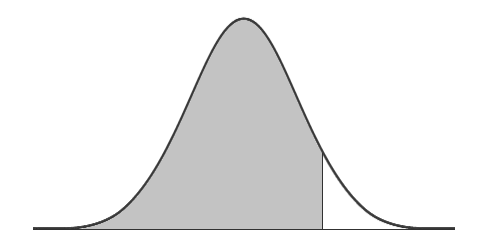
\includegraphics[width=\linewidth, right]{quantile}
			\captionsetup{labelformat=empty}
			\put (-28,32) {$\displaystyle \Phi(u_\beta) = \beta $}
			\put (-38,22) {\large $\swarrow$}
			\put (-33,-5) {$\displaystyle u_\beta $}
		\end{minipage}
	\end{center}
	\[\varphi^*(x) = 1_{\{\overline{X}_n > \mu_0 + u_{1-\alpha} \frac{\sigma}{\sqrt{n}}  \} }. \]
\end{exmp}

\begin{exmp} \label{exmp6.18}
	 Пусть $X_1, \dots X_n$ i.i.d. $\sim \mathcal{U}[0, \vartheta]$ и мы проверяем
	 \[ H:\vartheta=\vartheta_0 \quad \text{против} \quad K:\vartheta = \vartheta_1, \]
	 где $\vartheta_0 < \vartheta_1$. Плотности:
	 \[p_j(x) = \Big(\frac{1}{\vartheta_j}\Big)^n 1_{[0, \vartheta_j]} (x_{(n)}), \quad j=0,1, \]
	 и их отношение правдоподобия:
	 \[ \frac{p_1(x)}{p_0(x)}=
	 \left \{
	 \begin{array}{cl}
	 \Big(\frac{\vartheta_0}{\vartheta_1}\Big)^n, & x_{(n)} \leq \vartheta_0, \\
	 \infty, & x_{(n)} \in (\vartheta_0, \vartheta_1], \\
	 \text{произвольное}, & \text{иначе}.
	 \end{array}
	 \right.
	 \]
	 Далее
	 \[\alpha(c)  = P_{\vartheta_0}(p_1(X) > cp_0(X)) = 
	 \left \{
	 \begin{array}{cl}
	 1, & c \leq \Big(\frac{\vartheta_0}{\vartheta_1}\Big)^n, \\
	 0, & c > \Big(\frac{\vartheta_0}{\vartheta_1}\Big)^n.
	 \end{array}
	 \right.
	 \]
	 Для любого $\alpha \in (0, 1)$ имеет место
	 \[ \alpha(c) \leq \alpha \leq \alpha(c-) \quad \Longleftrightarrow \quad c = c^* = \Big(\frac{\vartheta_0}{\vartheta_1}\Big)^n.  \]
	 NP лемма гласит, что
	 \[ \varphi^*(x)=1_{\big\{\frac{p_1(x)}{p_0(x)} > c^*\big \}} + \gamma(x)1_{\big\{\frac{p_1(x)}{p_0(x)} = c^*\big \}} = 1_{\{x_{(n)}>\vartheta_0\}} + \gamma(x)1_{\{x_{(n)} \leq \vartheta_0\}}. \]
	 Как выбрать $\gamma(x)$? Возможностей много:
	 \[
	 \begin{aligned}
	 \varphi_1(x) = & 1_{\{x_{(n)} > c_1\}}, \quad c_1 = \vartheta_0 \sqrt[n]{1-\alpha}, \\
	 \varphi_2(x) = & 1_{\{x_{(n)} > \vartheta_0\}} + 1_{\{x_{(n)} < c_2\}}, \quad c_2 = \vartheta_0 \sqrt[n]{\alpha}, \\
	 \varphi_3(x) = & 1_{\{x_{(n)} > \vartheta_0\}} + \alpha1_{\{x_{(n)} \leq \vartheta_0\}}.
	 \end{aligned}
	 \]
\end{exmp}

\begin{rmrk}
	Простые гипотезы на практике не актуальны, но
	\begin{enumerate}
		\item Они дают интуитивное ощущение того, как нужно строить критерии. Во-первых, нужен т.н. \textbf{\textit{доверительный интервал}} $c(X) \subset \Theta$, внутри которого неизвестный параметр лежит с вероятностью $1-\alpha$. В Примере \ref{exmp6.17} мы использовали, что для $c(X)=[\overline{X}_n -u_{1 - \alpha} \frac{\sigma}{\sqrt{n}}, \infty)$ имеет место
		\[P_{\mu_0}(\mu_0 \in c(X)) = P_{\mu_0}(\overline{X}_n \leq \mu_0 + \frac{\sigma}{\sqrt{n}} u_{1-\alpha}) = 1-\alpha. \]
		Любой такой интервал  $c(X)$ может быть использован для построения критерия, например:
		\[c'(X) =\Big[\overline{X}_n -u_{1-\frac{\alpha}{2}} \frac{\sigma}{\sqrt{n}}, \overline{X}_n + u_{1-\frac{\alpha}{2}} \frac{\sigma}{\sqrt{n}} \Big].\]
		В дополнение, простые гипотезы показывают в какой стороне лежит альтернатива, и поэтому был выбран интервал $c(X)$ в Примере \ref{exmp6.17}.
		\item С помощью формальных результатов, таких как NP лемма, можно вывести более актуальные результаты.
	\end{enumerate}
\end{rmrk}

\begin{defn}
	Пусть $\Theta \subset \MR$, $\mathcal{P} = \{P_\vartheta\ |\ \vartheta \in \Theta \}$ и $T:(\mathcal{X},\mathcal{B}) \rightarrow (\MR,\mathcal{B})$ -- статистика. Семейство $\mathcal{P}$ называется \textbf{\textit{классом с монотонным (изотоническим) отношением правдоподобия}}, если для любого $\vartheta < \vartheta_1$ существует монотонно возрастающая функция $H_{\vartheta_0, \vartheta_1}: \MR \rightarrow [0, \infty)$, такая что
	\[\frac{p_{\vartheta_1}(x)}{p_{\vartheta_0}(x)} =H_{\vartheta_0, \vartheta_1}(T(x)) \quad P_{\vartheta_0} + P_{\vartheta_1}\text{-п.н.} \]
\end{defn}

\begin{exmp} \
	\begin{enumerate}
		\item В Примере \ref{exmp6.17}
		\[ \frac{p_{\mu_1}(x)}{p_{\mu_0}(x)} = \exp \Big \{ \frac{1}{\sigma^2} \sum_{i=1}^{n} x_i(\mu_1 - \mu_0) \Big \} \cdot f(\sigma^2, \mu_1, \mu_0),  \]
		монотонно возрастает по $\overline{X}_n$. Это свойство может быть обобщено до однопараметрических экспоненциальных семейств.
		\item В Примере \ref{exmp6.18}
		\[ \frac{p_{\vartheta_1}(x)}{p_{\vartheta_0}(x)} = \Big( \frac{\vartheta_0}{\vartheta_1} \Big)^n 1_{[0, \vartheta_0]}(x_{(n)}) + \infty 1_{(\vartheta_0, \vartheta_1]}(X_{(n)}) \]
		монотонно возрастает по $X_({n})$.
	\end{enumerate}
\end{exmp}

\begin{thm} \label{thm6.22}
	Пусть $\mathcal{P} = \{ P_\vartheta\ |\ \vartheta \in \Theta \}$ -- класс с монотонным отношением правдоподобия по $T$, $\vartheta_0 \in \Theta$ и  $\alpha \in (0, 1)$. Также, пусть
		\begin{center}\centering
			\begin{minipage}{0.7\textwidth}
				\[ \varphi^*(x) = 1_{\{T(x) > c\}} + \gamma 1_{\{ T(x) = c\}}, \]
				где
				\[ c := \inf \{t\ |\ P_{\vartheta_0}(T(X) > t) \leq \alpha \} \]
				и
				\[\gamma = 
				\left \{
				\begin{array}{cl}
				\frac{\alpha - P_{\vartheta_0}(T(X) > c) }{ P_{\vartheta_0}(T(X) = c) }, & \text{если } P_{\vartheta_0}(T(X) = c) \neq 0  \\
				0, & \text{иначе}.
				\end{array}
				\right.
				\]
			\end{minipage}
			\begin{minipage}{0.18\textwidth}
				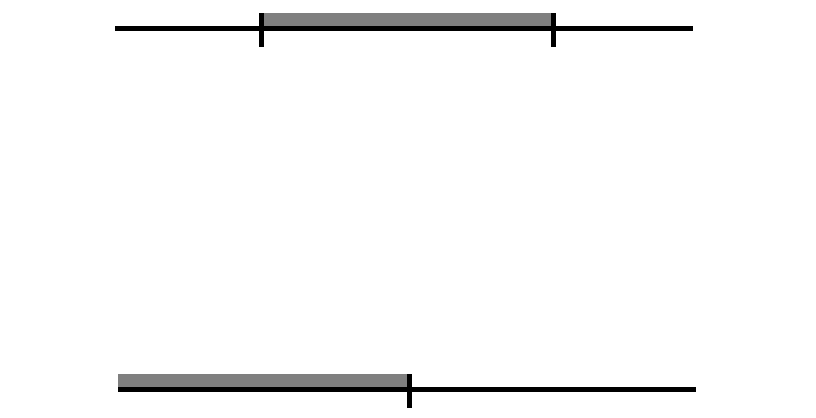
\includegraphics[width=\linewidth, right]{hypotheses}
				\captionsetup{labelformat=empty}
				\put (-105,10) {односторонние гипотезы:}
				\put (-30,-8) {$\displaystyle K$}
				\put (-65,-8) {$\displaystyle H$}
				\put (-103,50) {двусторонние гипотезы:}
				\put (-48,30) {$\displaystyle H$}
				\put (-75,30) {$\displaystyle K$}
				\put (-25,30) {$\displaystyle K$}
			\end{minipage}
		\end{center}
	Тогда 
	\begin{enumerate}
		\item $\beta_{\varphi^*}(\vartheta_0) = \alpha$ и $\varphi^*$ -- UMP-критерий с уровнем значимости $\alpha$ для односторонних гипотез:
		\[ H:\vartheta \leq \vartheta_0 \quad \text{против} \quad K:\vartheta > \vartheta_0. \]
		\item Для любого $\vartheta < \vartheta_0$ имеет место равенство
		\[ \beta_{\varphi^*}(\vartheta) = \inf \{ \beta_\varphi(\vartheta)\ |\ \varphi \in \Phi \text{ и } \beta_\varphi(\vartheta_0) = \alpha \}. \]
		\item Функция мощности $\vartheta \mapsto \beta_{\varphi^*}(\vartheta)$ строго монотонно возрастает для любого $\vartheta$, такого что $\beta_{\varphi^*}(\vartheta) \in (0,1)$.
		\item Для любого $\vartheta' \in \Theta$ $\varphi^*$ -- UMP-критерий с уровнем значимости $\alpha' = \ME_{\vartheta'}[\varphi^*(X)]$ для гипотез
		\[H': \vartheta \leq \vartheta' \quad \text{против} \quad K': \vartheta > \vartheta'. \]
    \end{enumerate}
\end{thm}
\begin{proof} \
	\begin{enumerate}
		\item Если $P_{\vartheta_0}(T(X) = c) = 0$, то
		\[\beta_{\varphi^*}(\vartheta_0) = P_{\vartheta_0}(T(X) > c) = \alpha.  \]
		Если $P_{\vartheta_0}(T(X) = c) > 0$, то мы подбираем $\gamma$ таким образом, чтобы имело место равенство
		\[\beta_{\varphi^*}(\vartheta_0)=P_{\vartheta_0}(T(X)>c) + \gamma P_{\vartheta_0}(T(X) = c) = \alpha. \]
		Пусть $\vartheta_0 < \vartheta_1$ и $H_{\vartheta_0, \vartheta_1}(T(x)) = p_{\vartheta_1}(x) / p_{\vartheta_0}(x)$. Вследствие монотонности
		\[ H_{\vartheta_0, \vartheta_1}(T(x)) \lessgtr H_{\vartheta_0, \vartheta_1}(c) = s \quad \Longrightarrow \quad T(x) \lessgtr c \]
		и
		\[ \varphi^*(x) =
		\left \{
		\begin{array}{cl}
		1, & H_{\vartheta_0, \vartheta_1}(x) > s, \\
		0, & H_{\vartheta_0, \vartheta_1}(x) < s.
		\end{array}
		\right.
	    \]
	    Таким образом $\varphi^*$ -- NP критерий с уровнем значимости $\alpha$ и по NP лемме
	    \[ \beta_{\varphi^*}(\vartheta') = \sup \{\beta_\varphi(\vartheta_1)\ |\ \varphi \in \Phi \text{ и } \beta_\varphi(\vartheta_0) = 1-\alpha \}. \]
	    Так как $\varphi^*$ не зависит от выбора $\vartheta_1$, это соотношение имеет место для любого $\vartheta_1 > \vartheta_0$. Наконец, пусть $\varphi'(x) = 1 - \varphi^*(x)$. Используя те же рассуждения, что и выше, можно показать, что
	    \[ \beta_{\varphi'}(\vartheta_2) = \sup \{\beta_\varphi(\vartheta_2)\ |\ \varphi \in \Phi \text{ и } \beta_\varphi(\vartheta_0) = \alpha \} \quad \forall \vartheta_2 < \vartheta_0. \]
	    Так как критерий вида $\overline{\varphi} \equiv \alpha$ удовлетворяет равенству $\beta_{\overline{\varphi}}(\vartheta_0) = \alpha$, мы заключаем, что
	    \[1 - \beta_{\varphi^*}(\vartheta_2) = \beta_{\varphi'}(\vartheta_2) \geq \beta_{1-\overline{\varphi}}(\vartheta_2) = 1 -\beta_{\overline{\varphi}}(\vartheta_2) = 1 - \alpha.   \]
	    Следовательно, $\beta_{\varphi^*}(\vartheta_2) \leq \alpha$ и $\varphi^* \in \Phi_\alpha$.
		\item Утверждение следует непосредственно, так как $\beta_{\varphi'} = 1 - \beta_{\varphi^*}$.
		\item Следует из Следствия \ref{crlr6.16}, так как для любых $\vartheta_1 < \vartheta_2$ $\varphi^*$ -- NP критерий.
		\item Доказывается, используя схожие аргументы, что и в доказательстве пункта (i).
	\end{enumerate}
\end{proof}

\begin{exmp}
	Пусть $X_1, \dots X_n$ i.i.d. $\sim \mathcal{N}(\mu, \sigma^2)$ с известным параметром $\sigma^2$. Из Примера \ref{exmp6.17} мы знаем, что плотности
	\[p_\mu(x) = (2 \pi \sigma^2)^{-\frac{n}{2}} \exp \Big\{ -\frac{1}{2\sigma^2}\sum_{i=1}^{n}(x_i - \mu)^2 \Big\} \]
	обладают монотонным отношением правдоподобия по $T(x) = \overline{x}_n$. Из Теоремы \ref{thm6.22}: UMP-критерий с уровнем значимости $\alpha$ для
	\[ H:\mu \leq \mu_0 \quad \text{против} \quad K:\mu > \mu_0  \]
	имеет вид
	\[ \varphi^*(x) = 1_{\{\overline{x}_n > c\}} + \gamma 1_{\{\overline{x}_n = c\}}. \]
	Так как $P_{\mu_0}(T(X) = c) = 0$, то $\gamma = 0$ и выбрать $c$ так, что $P_{\mu_0}(\overline{X}_n > c) = \alpha \Longleftrightarrow c = \mu_0 + \frac{\sigma}{\sqrt{n}} u_{1-\alpha}$. UMP-критерий
	\[ \varphi^*(x) = 1_{\{\overline{X}_n > \mu_0 + \frac{\sigma}{\sqrt{n}}u_{1-\alpha} \} } \]
	называется \textbf{\textit{односторонним критерием Гаусса}}.
\end{exmp}

\begin{rmrk} \
	\begin{enumerate}
		\item Существует эвристика, как получить односторонний критерий Гаусса: так как $\overline{X}_n$ UMVU-оценка для $\mu$, разумной стратегией будет принятие гипотезы $K$, если $\overline{X}_n$ достаточно большое. Следовательно, критерий должен иметь вид:
		\[\varphi(x) = 1_{\{\overline{X}_n > c\}}.  \]
		Выбираем $c$, контролируя вероятность ошибки первого рода. Для любого $\mu \leq \mu_0$ имеет место
		\[ \beta_\varphi(\mu) = P_\mu(\overline{X}_n > c) = P_\mu \Big( \frac{\sqrt{n}(\overline{X}_n - \mu) }{\sigma} > \frac{\sqrt{n}(c-\mu)}{\sigma}\Big) = 1 - \Phi\Big(\frac{\sqrt{n}(c-\mu)}{\sigma}\Big) \leq 1 - \Phi\Big(\frac{\sqrt{n}(c-\mu_0)}{\sigma}\Big).\]
		Мы должны удостовериться, что:
		\[ 1- \Phi\Big(\frac{\sqrt{n}(c-\mu_0)}{\sigma}\Big) \leq \alpha, \]
		иначе говоря:
		\[c \geq \mu_0 + \frac{\sigma}{\sqrt{n}} u_{1-\alpha}.\] 
		Мы берем $c = \mu_0 + \frac{\sigma}{\sqrt{n}} u_{1-\alpha}$, чтобы вероятность ошибки первого рода была равна $\alpha$.
		\item Этот метод позволяет построить критерий, однако ничего не говорит о его оптимальности. Что важно, он может быть применен в более общих ситуациях, например в случае неизвестного параметра $\sigma^2$. В такой ситуации можно воспользоваться оценкой
		\[ \hat{\sigma}_n^2 = \frac{1}{n-1}\sum_{i=1}^{n}(X_i - \overline{X}_n)^2. \]
		Как и выше, мы получаем:
		\[ \beta_\varphi(\mu) = P_\mu\Big( \frac{\sqrt{n}(\overline{X}_n - \mu) }{\hat{\sigma}_n} > \frac{\sqrt{n}(c-\mu)}{\hat{\sigma}_n}\Big) = 1 - F_{t_{n-1}}\Big( \frac{c - \mu}{\sqrt{\hat{\sigma}_n^2 / n}} \Big)  \]
		из Следствия \ref{crlr2.21}, где $F_{t_{n-1}}$ -- функция распределения $t_{n-1}$. Разумный выбор константы:
		\[ c = \mu_0 + \frac{\hat{\sigma}_n}{\sqrt{n}}t_{n-1,1-\alpha}, \]
		где $t_{n-1, 1-\alpha}$ -- $1-\alpha$-квантиль распределения Стьюдента с $n-1$ степенями свободы. Критерий
		\[ 1_{\{ \overline{x}_n > \mu_0 + \frac{\hat{\sigma}_n}{\sqrt{n}}t_{n-1,1-\alpha} \}} \]
		называется \textbf{\textit{односторонним t-критерием}}.
	\end{enumerate}
\end{rmrk}

\begin{rmrk}
	В общем случае не существует UMP-критериев для
	\[ H:\vartheta = \vartheta_0 \quad \text{против} \quad K:\vartheta \neq \vartheta_0, \]
	так как этот критерий должен быть оптимальным для всех
	\[ H':\vartheta = \vartheta_0 \quad \text{против} \quad K':\vartheta = \vartheta_1, \]
	где $\vartheta_0 \neq \vartheta_1$.
	В случае монотонного отношения правдоподобия оптимальный критерий будет
	\[ \varphi(x) = 1_{\{ T(x) > c \}} + \gamma(x) 1_{\{T(x) = c\}} \]
	для $\vartheta_1 > \vartheta_0$ и
	\[ \varphi'(x) = 1_{\{ T(x) < c'\}} + \gamma'(x) 1_{\{T(x) = c'\}} \]
	для $\vartheta_1 < \vartheta_0$, что невозможно.
\end{rmrk}

\begin{thm} \label{thm6.26}
	Пусть $\mathcal{P} = \{ P_\vartheta\ |\ \vartheta \in \Theta \}$ -- однопараметрическое экспоненциальное семейство с $\mu$-плотностью
	\[p_\vartheta(x) = c(\vartheta)h(x)\exp(Q(\vartheta) T(x)) \]
	с возрастающей функцией $Q$. Тогда существует UMPU-критерий для
	\[ H:\vartheta \in [\vartheta_1, \vartheta_2] \quad \text{против} \quad K:\vartheta \notin [\vartheta_1, \vartheta_2], \]
	а именно
	\[ \varphi^*(x) = 
	\left \{
	\begin{array}{cl}
	1, & \text{если } T(x) \notin [c_1, c_2], \\
	\gamma_i, & \text{если } T(x) = c_i, \\
	0, & \text{если } T(x) \in (c_1, c_2),
	\end{array}
	\right.
	\]
	где константы $c_i$, $\gamma_i$ определяются из равенства
	\[ \beta_\varphi(\vartheta_1) = \beta_\varphi(\vartheta_2) = \alpha \]
\end{thm}
\begin{proof}
	Теорема 3.7.1 в \cite{LehmannRomano}.
\end{proof}

\begin{rmrk}
	Похожие утверждения имеют место для $k$-параметрических экспоненциальных семейств.
\end{rmrk}

\raggedbottom
\pagebreak

\section*{Упражнения}
\begin{exc}
	Пусть $X_1, \dots, X_n$ -- i.i.d. нормально распределенные случайные величины: $X_i \sim \mathcal{N}(\mu, \sigma^2)$ с известным математическим ожиданием $\mu \in \MR$ и неизвестной дисперсией $\sigma^2 > 0$. Постройте UMP-критерий с уровнем значимости $\alpha \in (0, 1)$ для гипотез
	\[H: \sigma^2 < \sigma_0^2 \quad \text{против} \quad K:\sigma \geq \sigma_0^2.  \]
\end{exc}

\begin{exc}
	Пусть мы наблюдаем $X \in (0, 1)$. Постройте UMP-критерий с уровнем значимости $\alpha$ для
	\[H:\text{плотность $X$: } f(x) = 4x1_{(0, 1/2)}(x) + (4 - 4x)1_{(1/2, 1)}(x) \]
	против альтернативы
	\[ K: X \sim \mathcal{U}(0, 1).\]
\end{exc}

\begin{exc}
	Пусть $X$ -- случайная величина с плотностью
	\[ f_\vartheta(x) = \frac{2(\vartheta - x)}{\vartheta^2}1_{(0, \vartheta)}(x). \]
	Постройте UMP-критерий с уровнем значимости $\alpha$ для гипотез
	\[H: \vartheta = \vartheta_0 \quad \text{против} \quad K:\vartheta = \vartheta_1 \]
	для $\vartheta_1 < \vartheta_0$.
\end{exc}

\begin{exc} \label{exc6.4}
	Пусть $X_1, \dots, X_n$ -- i.i.d. экспоненциально распределенные случайные величины: $X_i \sim Exp(\vartheta)$, т.е. плотность $X_i$:
	\[ f_\vartheta(x) = \vartheta \exp (\vartheta x) 1_{[0, \infty)}(x).  \]
	\begin{enumerate}
		\item Покажите, что распределение $X = (X_1, \dots, X_n)$ обладает мононотонным отношением правдоподобия.
		\item Постройте UMP-критерий для гипотез
		\[H: \vartheta < \vartheta_0 \quad \text{против} \quad K:\vartheta \geq \vartheta_0.  \]
		\item Рассчитайте критическую область для этого критерия для $\vartheta_0 = 1$, $n = 10$ и $\alpha = 0.05$.
		\subitem \textit{Подсказка}: 5\%-квантиль гамма распределения $\Gamma(10, 1)$ приблизительно равен 5.43.
		\end{enumerate}
\end{exc}

\begin{exc}
	Рассмотрим еще раз ситуацию из Упражнения \ref{exc6.4}.
	\begin{enumerate}
		\item Рассмотрим гипотезы
		\[ H:\vartheta = \vartheta_0 \quad \text{против} \quad K:\vartheta \neq \vartheta_0. \]
		Обрисуйте построение доверительного интервала $[\overline{X}_n - \alpha, \overline{X}_n + \alpha]$ с уровнем значимости $\alpha$ для $\gamma(\vartheta) = 1/ \vartheta$. Как он поможет для построения критерия для гипотез выше?
		\item Используйте аппроксимацию нормальным распределением, чтобы построить доверительный интервал из (i) для $n=100$ и $\alpha = 0.1$.
	\end{enumerate}
\end{exc}

\begin{exc}
	Продолжим рассмотрение Упражнения \ref{exc6.4}.
	\begin{enumerate}
		\item Пусть $n=1$. Постройте UMPU-критерий с уровнем значимости $\alpha$ для гипотез
		 \[ H:\vartheta \in [1, 2] \quad \text{против} \quad K:\vartheta \notin [1, 2].  \]
		 \item Теоретически мы можем воспользоваться Теоремой \ref{thm6.26}, чтобы построить UMPU-критерий для гипотез
		 \[ H:\vartheta = \vartheta_0 \quad \text{против} \quad K:\vartheta \neq \vartheta_0.  \]
		 Какие проблемы могут возникнуть? Как их можно обойти?
	\end{enumerate}
\end{exc}